\part{Einleitung}
\label{part:intro}

\begin{frame}[fragile]{}
Einleitung!
\end{frame}

\part{HoloLens}
\label{part:hololens}
\begin{frame}[fragile]{}
\begin{figure}[h!]
	\centering
	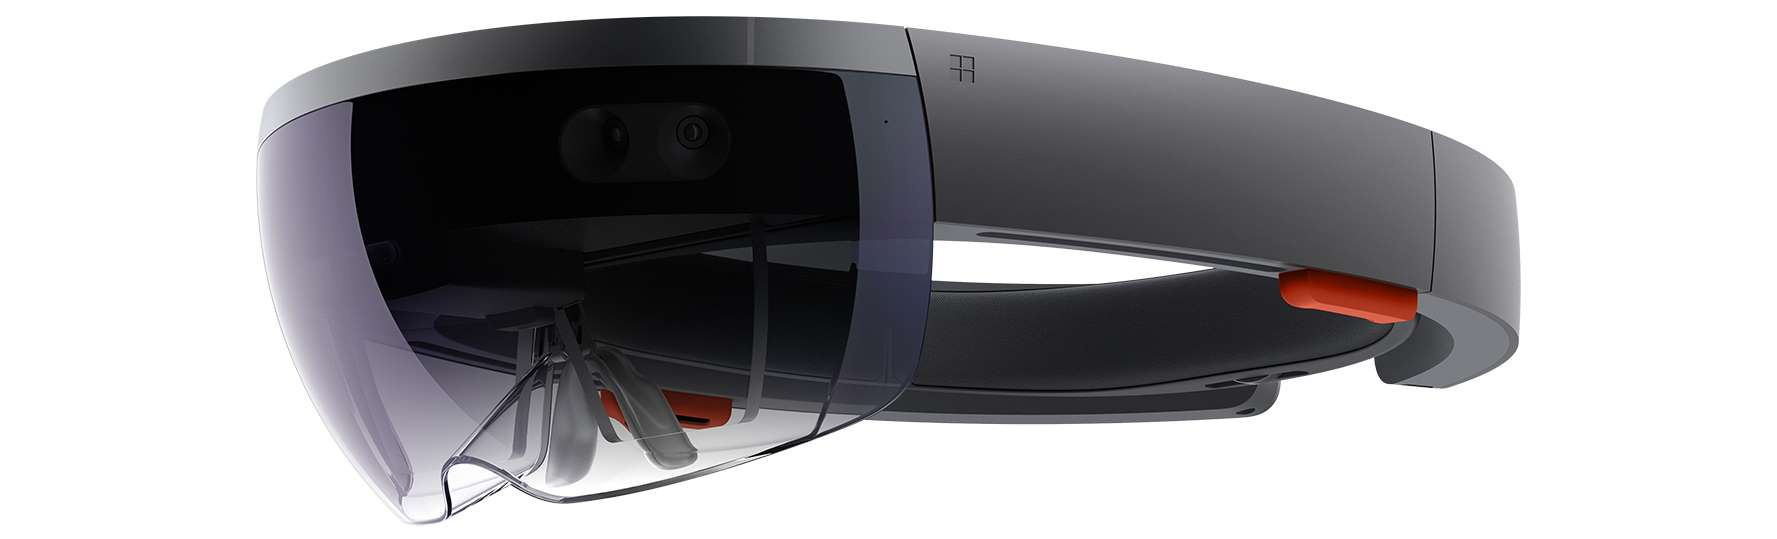
\includegraphics[width=0.7\textwidth]{images/hololens.jpg}
\end{figure}
\begin{itemize}
	\pause
	\item \textit{Mixed Reality} Device
	\pause
	\item Projeziert virtuelle Objekte in das Sichtfeld des Nutzers
	\pause
	\item Nutzer bewegt sich simultan durch reale und virtuelle Szene
	\pause
	\item Genaue Bestimmung von Position und Ausrichtung im Raum durch Sensoren: \textit{Inside-Out-Tracking}
\end{itemize}	
\end{frame}

\begin{frame}[fragile]{HoloLens und Autodesk}
\begin{figure}[h!]
	\centering
	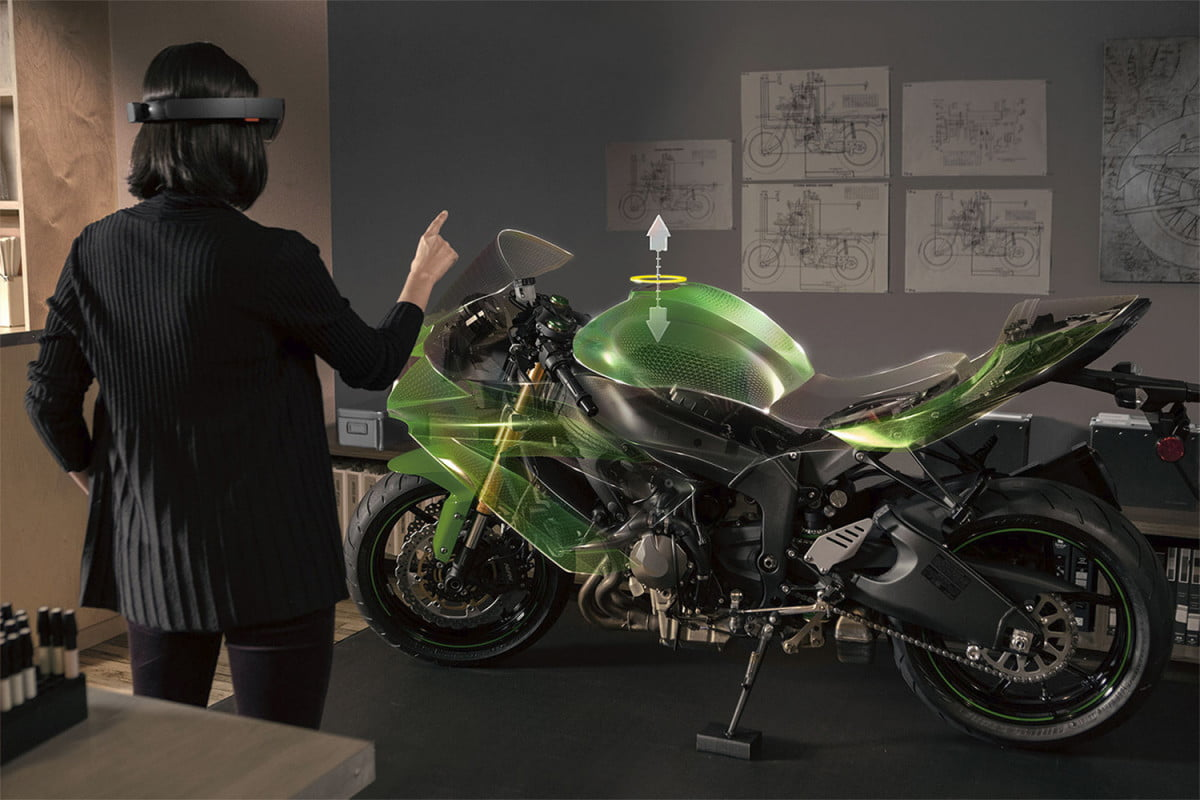
\includegraphics[width=0.75\textwidth]{images/HoloLens_Motorcycle.jpg}
	\setlength{\abovecaptionskip}{5pt plus 5pt minus 2pt}
	\caption*{Quelle: Digitaltrends}
\end{figure}
\end{frame}

\part{State of the Art}
\label{part:sota}
\begin{frame}[fragile]{HoloLens in der Physik}
\begin{figure}
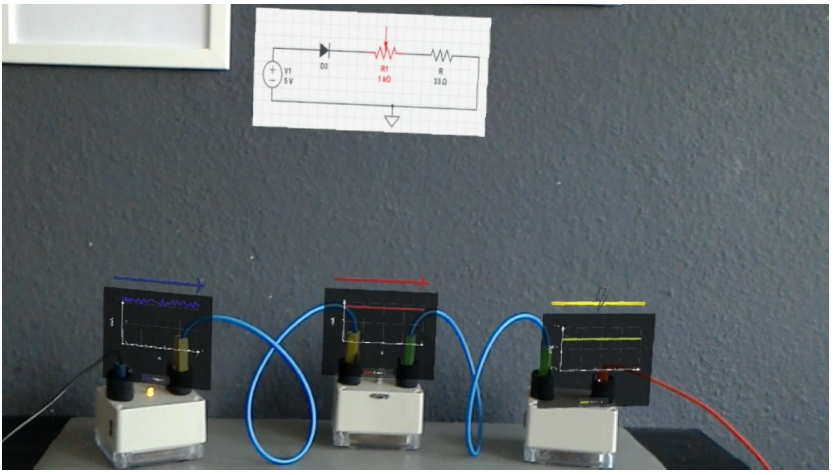
\includegraphics[width=0.43\textwidth]{images/Amiraslanov18.png}
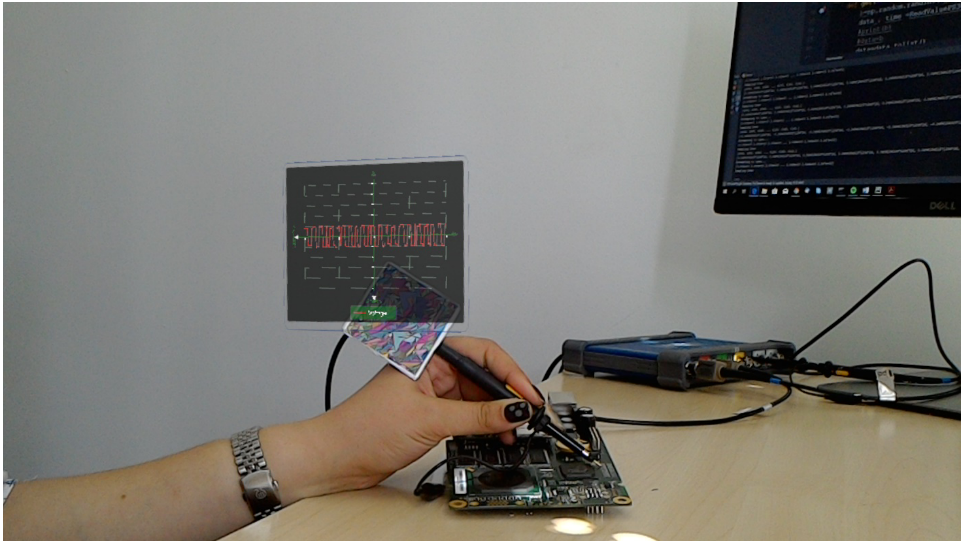
\includegraphics[width=0.43\textwidth]{images/Javaheri18.png}
\begin{center}
\vspace{0.05cm}
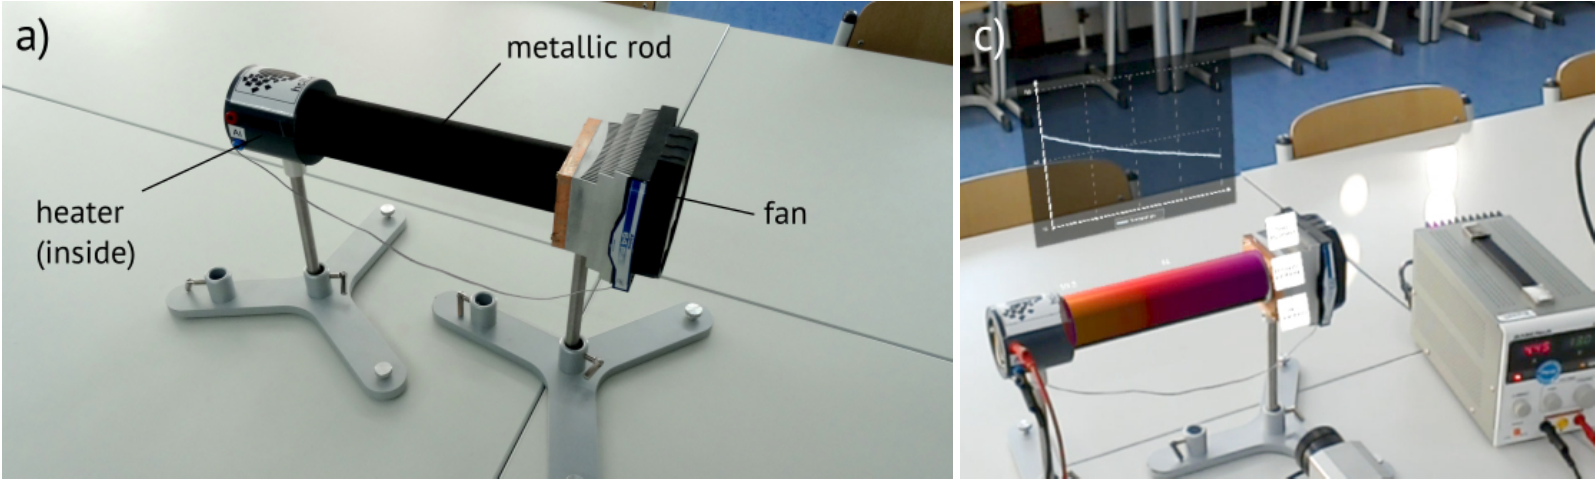
\includegraphics[width=0.87\textwidth]{images/Strzys18.png}	
\end{center}
\setlength{\abovecaptionskip}{7pt plus 5pt minus 2pt}
\caption*{Oben Links: \citep{Amiraslanov18}, Oben Rechts: \cite{Javaheri18}, Unten: \cite{Strzys18}}
\end{figure}

\end{frame}

\begin{frame}[fragile]{Mixed Reality in der Physik}

\begin{figure}
	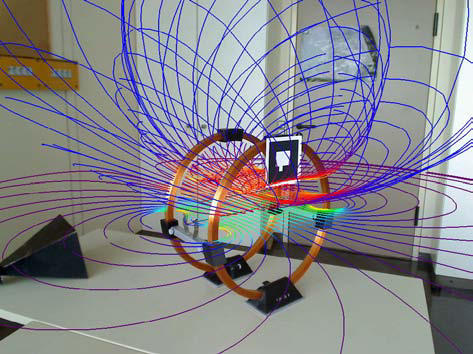
\includegraphics[width=0.35\textwidth]{images/Buchau09.jpg}
	\hspace{0.05cm}
	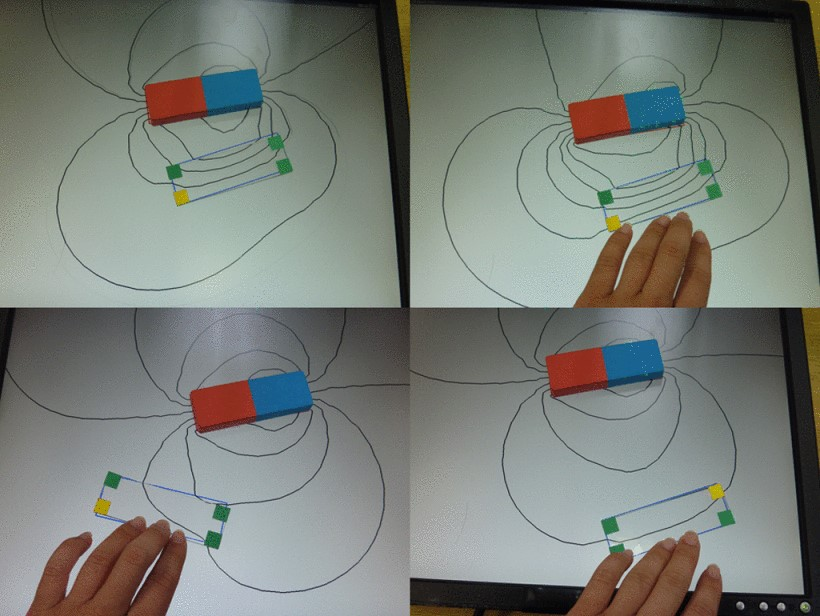
\includegraphics[width=0.35\textwidth]{images/Matsutomo13.jpg}

%	\centering
	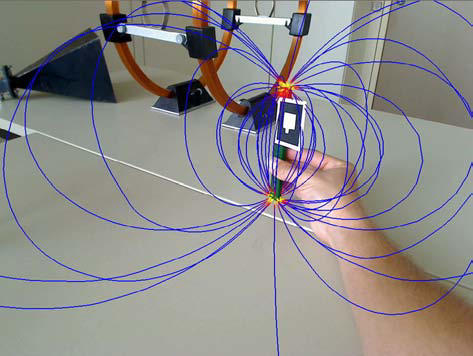
\includegraphics[width=0.35\textwidth]{images/Buchau09_Magnet.jpg}
	\hspace{0.05cm}
	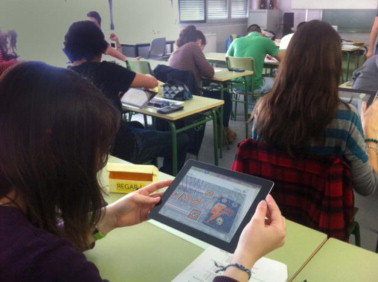
\includegraphics[width=0.35\textwidth]{images/Ibanez14.jpg}

	\setlength{\abovecaptionskip}{5pt plus 5pt minus 2pt}
	\caption*{Links: \citep{Buchau09}, Rechts Oben: \cite{Matsutomo13}, Rechts Unten: \cite{Ibanez14}}
\end{figure}
\end{frame}

\part{Anwendungsfall: Helmholtz-Spulen}
\label{part:physics}
\begin{frame}[fragile]{}
\begin{center}
	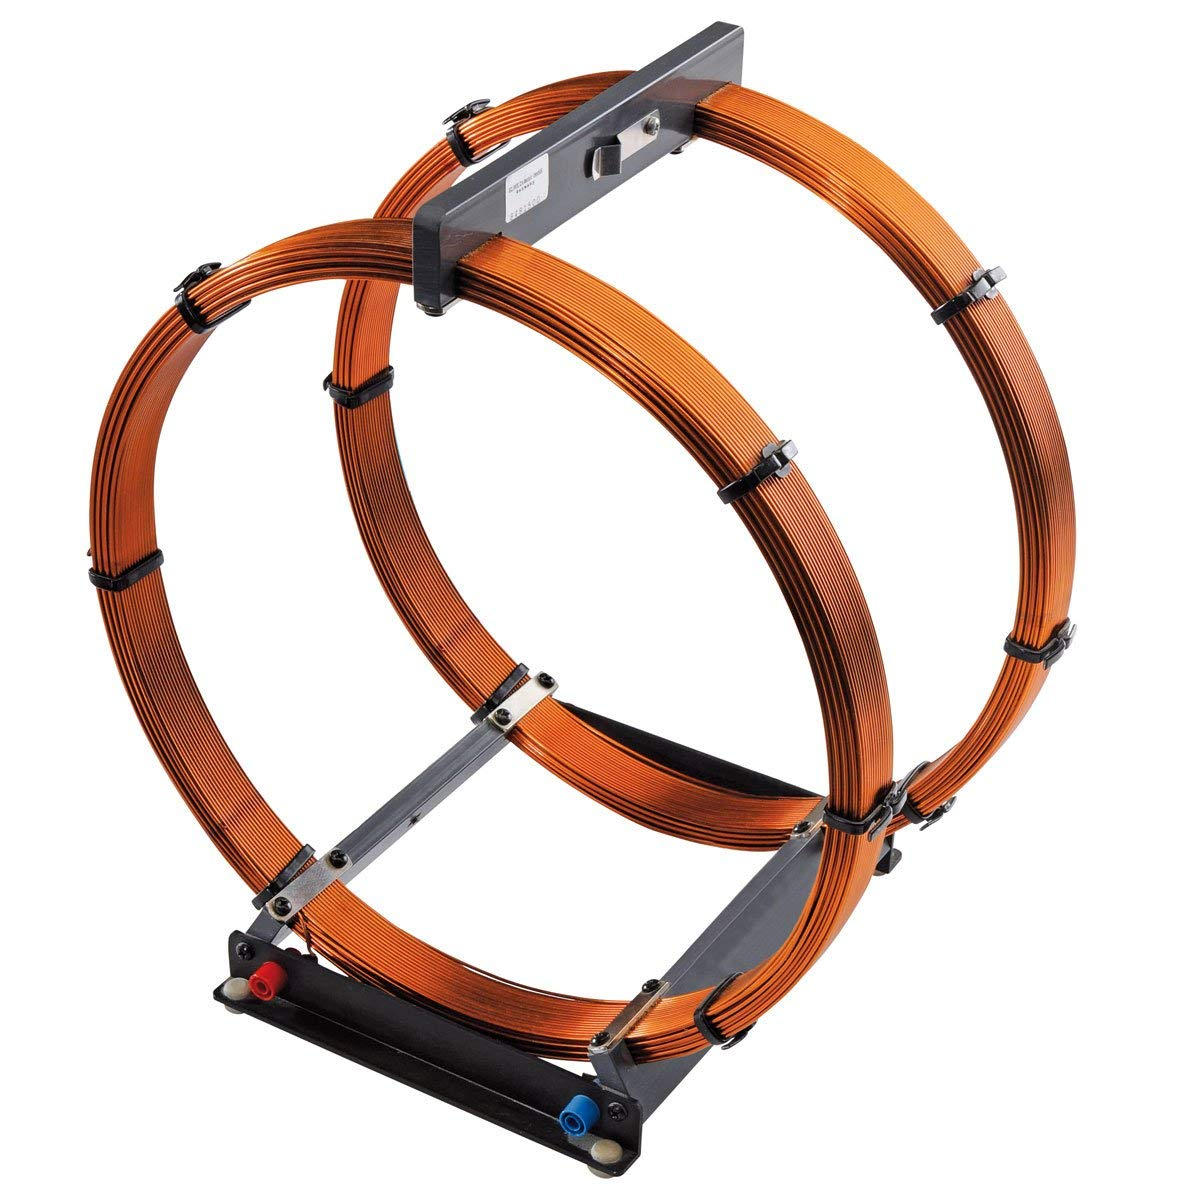
\includegraphics[width=0.5\textwidth]{images/Helmholtz.jpg}	
\end{center}
\end{frame}

\part{Ziel \& Frage}
\label{part:goal}
\begin{frame}[fragile]{}
\usebeamerfont{frametitle}\textcolor{blue}{Ziel:} \usebeamerfont{text}HoloLens einsetzen, um Versuchsaufbau mit Informationen anzureichern.
\pause
\vskip 1em
\usebeamerfont{frametitle}\textcolor{blue}{Frage:} \usebeamerfont{text}Wie kann die HoloLens für diesen Versuch konkret eingesetzt werden?
\end{frame}

\part{Anforderungen}
\begin{frame}[fragile]{}
\begin{center}
	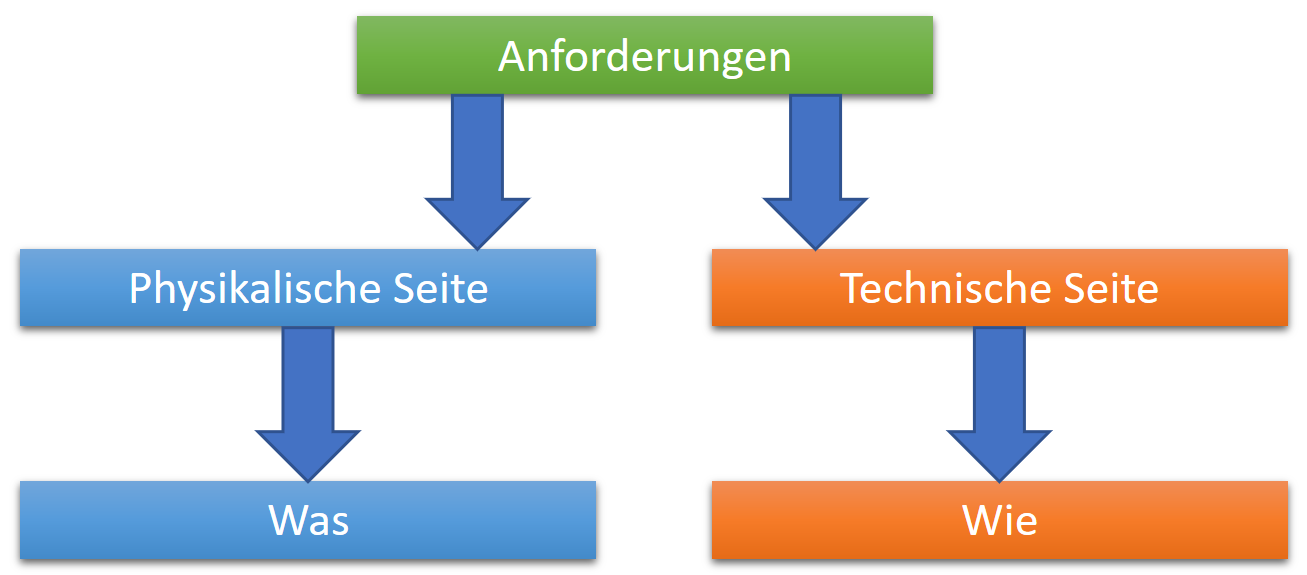
\includegraphics[width=0.9\textwidth]{images/Anforderungen.png}
\end{center}
\end{frame}

\part{Physikalische Seite}
\begin{frame}[fragile]{Anforderungen aus dem Anwendungsfall heraus}
\begin{itemize}
%	\setlength{\itemsep}{0.01\baselineskip}
	\item Magnetfeld von Erde und Spule
	\begin{itemize}
%		\setlength{\itemsep}{0.01\baselineskip}
		\item Stärke
		\item Richtung
		\item Homogenität
		\item Inhomogenität am Rand der Spule andeuten (Optional) 
	\end{itemize}
	\item Stromfluss durch die Spule
	\begin{itemize}
		\item Richtung
		\item Kennzeichnung von Plus und Minus
		\item Stärke (Optional) 
	\end{itemize}
\end{itemize}
\end{frame}

\begin{frame}[fragile]{Anforderungen aus dem Anwendungsbereich}
\begin{itemize}
	\setlength{\itemsep}{-0.25em}
	\item Kompass
	\begin{itemize}
		\setlength{\itemsep}{-0.25em}
		\item Nordrichtung
		\item Grobe Auslenkung der Nadel
	\end{itemize}
	\item Weitere Informationen (Optional)
	\begin{itemize}
		\item Windungszahl der Spule
		\item Durchmesser und Abstand der Spulen
		\item Numerische Werte und Informationen (z.B. Fließt aktuell Strom, angelegte Stromstärke, angenommene Stärke des Erdmagnetfeldes, systematischer und zufälliger Fehler, etc.)
	\end{itemize}
\end{itemize}
\end{frame}

\part{Technische Seite}
\label{part:tech}

\begin{frame}[fragile]{Eigenschaften der HoloLens}
\begin{itemize}
	\item \textit{See-Through Display}, stereoskopisch, Zwei 16:9 HD Bilder, 32\degree Field of View, \textit{Color Sequential Display}, 60 Hz Bildwiederholrate hochskaliert auf 240 Hz, Akkomodation der Augen fest bei 2 m
	\pause
	\begin{itemize}
		\item Für Objekte: Größe, Geschwindigkeit, Farbe, Distanz zur Kamera
		\pause
		\item Schwarz = Transparent, kein fester Hintergrund, Darstellungen überdecken Hintergrund, Helligkeit im Raum beeinflusst Darstellung
	\end{itemize}
	\pause
	\item \textit{Inside-Out Tracking} über Tiefenkamera (Infrarot), Stereo-Kameras und Inertialmesssystem (IMU)
	\begin{itemize}
		\pause
		\item 60 FPS stabil halten, stark spiegelnde oder transparente Oberflächen vermeiden, mögliche Einflüsse auf die Sensoren beachten
	\end{itemize}
\end{itemize}
\end{frame}

\begin{frame}[fragile]{Eigenschaften der HoloLens}
\begin{itemize}
	\item Stand-Alone Device, 1 GHz CPU, 1 GHz HPU, 2 GB RAM, 1 GB HPU RAM, passiv gekühlt
	\begin{itemize}
		\pause
		\item Strenges Performance Limit, keine rechenintensiven Anwendungen möglich, Akkulaufzeit, Qualitätseinschränkungen bei Mixed Reality Capture, etc.
	\end{itemize}
	\pause
	\item Interaktion über Handgesten und Sprache, Cursor = vorwärtsgerichteter Raycast im Zentrum des Sichtfeldes
	\item Usability und UX Einschränkungen bzw. Empfehlungen
\end{itemize}
\end{frame}


\part{Problemstellung}
\label{part:golas}
\begin{frame}
\vspace{-1em}
\begin{center}
	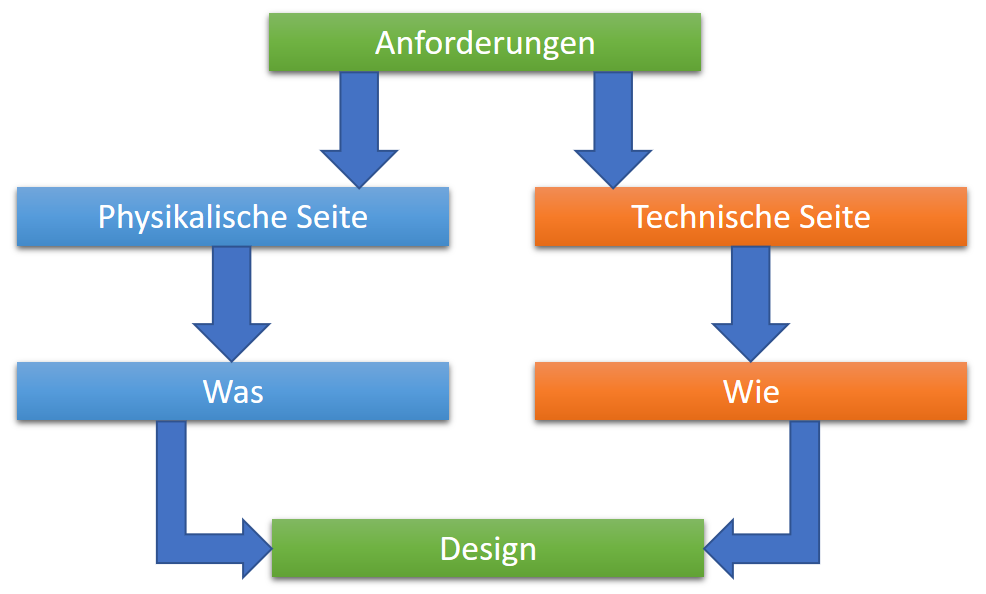
\includegraphics[width=0.8\textwidth]{images/Informiertes_Design.png}	
\end{center}
\usebeamerfont{frametitle}\textcolor{blue}{Fragen:}
\begin{itemize}
	\item Was soll dargestellt werden?
	\item Wie soll es dargestellt werden?
	\item Wie soll damit interagiert werden?
\end{itemize}
\vspace{50px}
\end{frame}


\part{Design}
\label{part:design}
\begin{frame}[fragile]{Ansatz -- Magnetfeld}
\begin{itemize}
	\item Magnetfeld als räumlich in die Spule eingebettete, dreidimensionale Geometrie anzeigen
	\item Zwei verschiedene schematische Darstellungen für Magnetfeld anbieten: Vektor-Modell und Feldlinien-Modell
	\item Einbettung durch Depth Cues unterstützen (in erster Linie Verdeckung der virtuellen Geometrie durch reale Spule)
	\item Sensordaten in Echtzeit an HoloLens übermitteln und Geometrie auf dem Device in Echtzeit berechnen und darstellen
\end{itemize}
\end{frame}

\begin{frame}
\vspace{-1em}
\begin{center}
	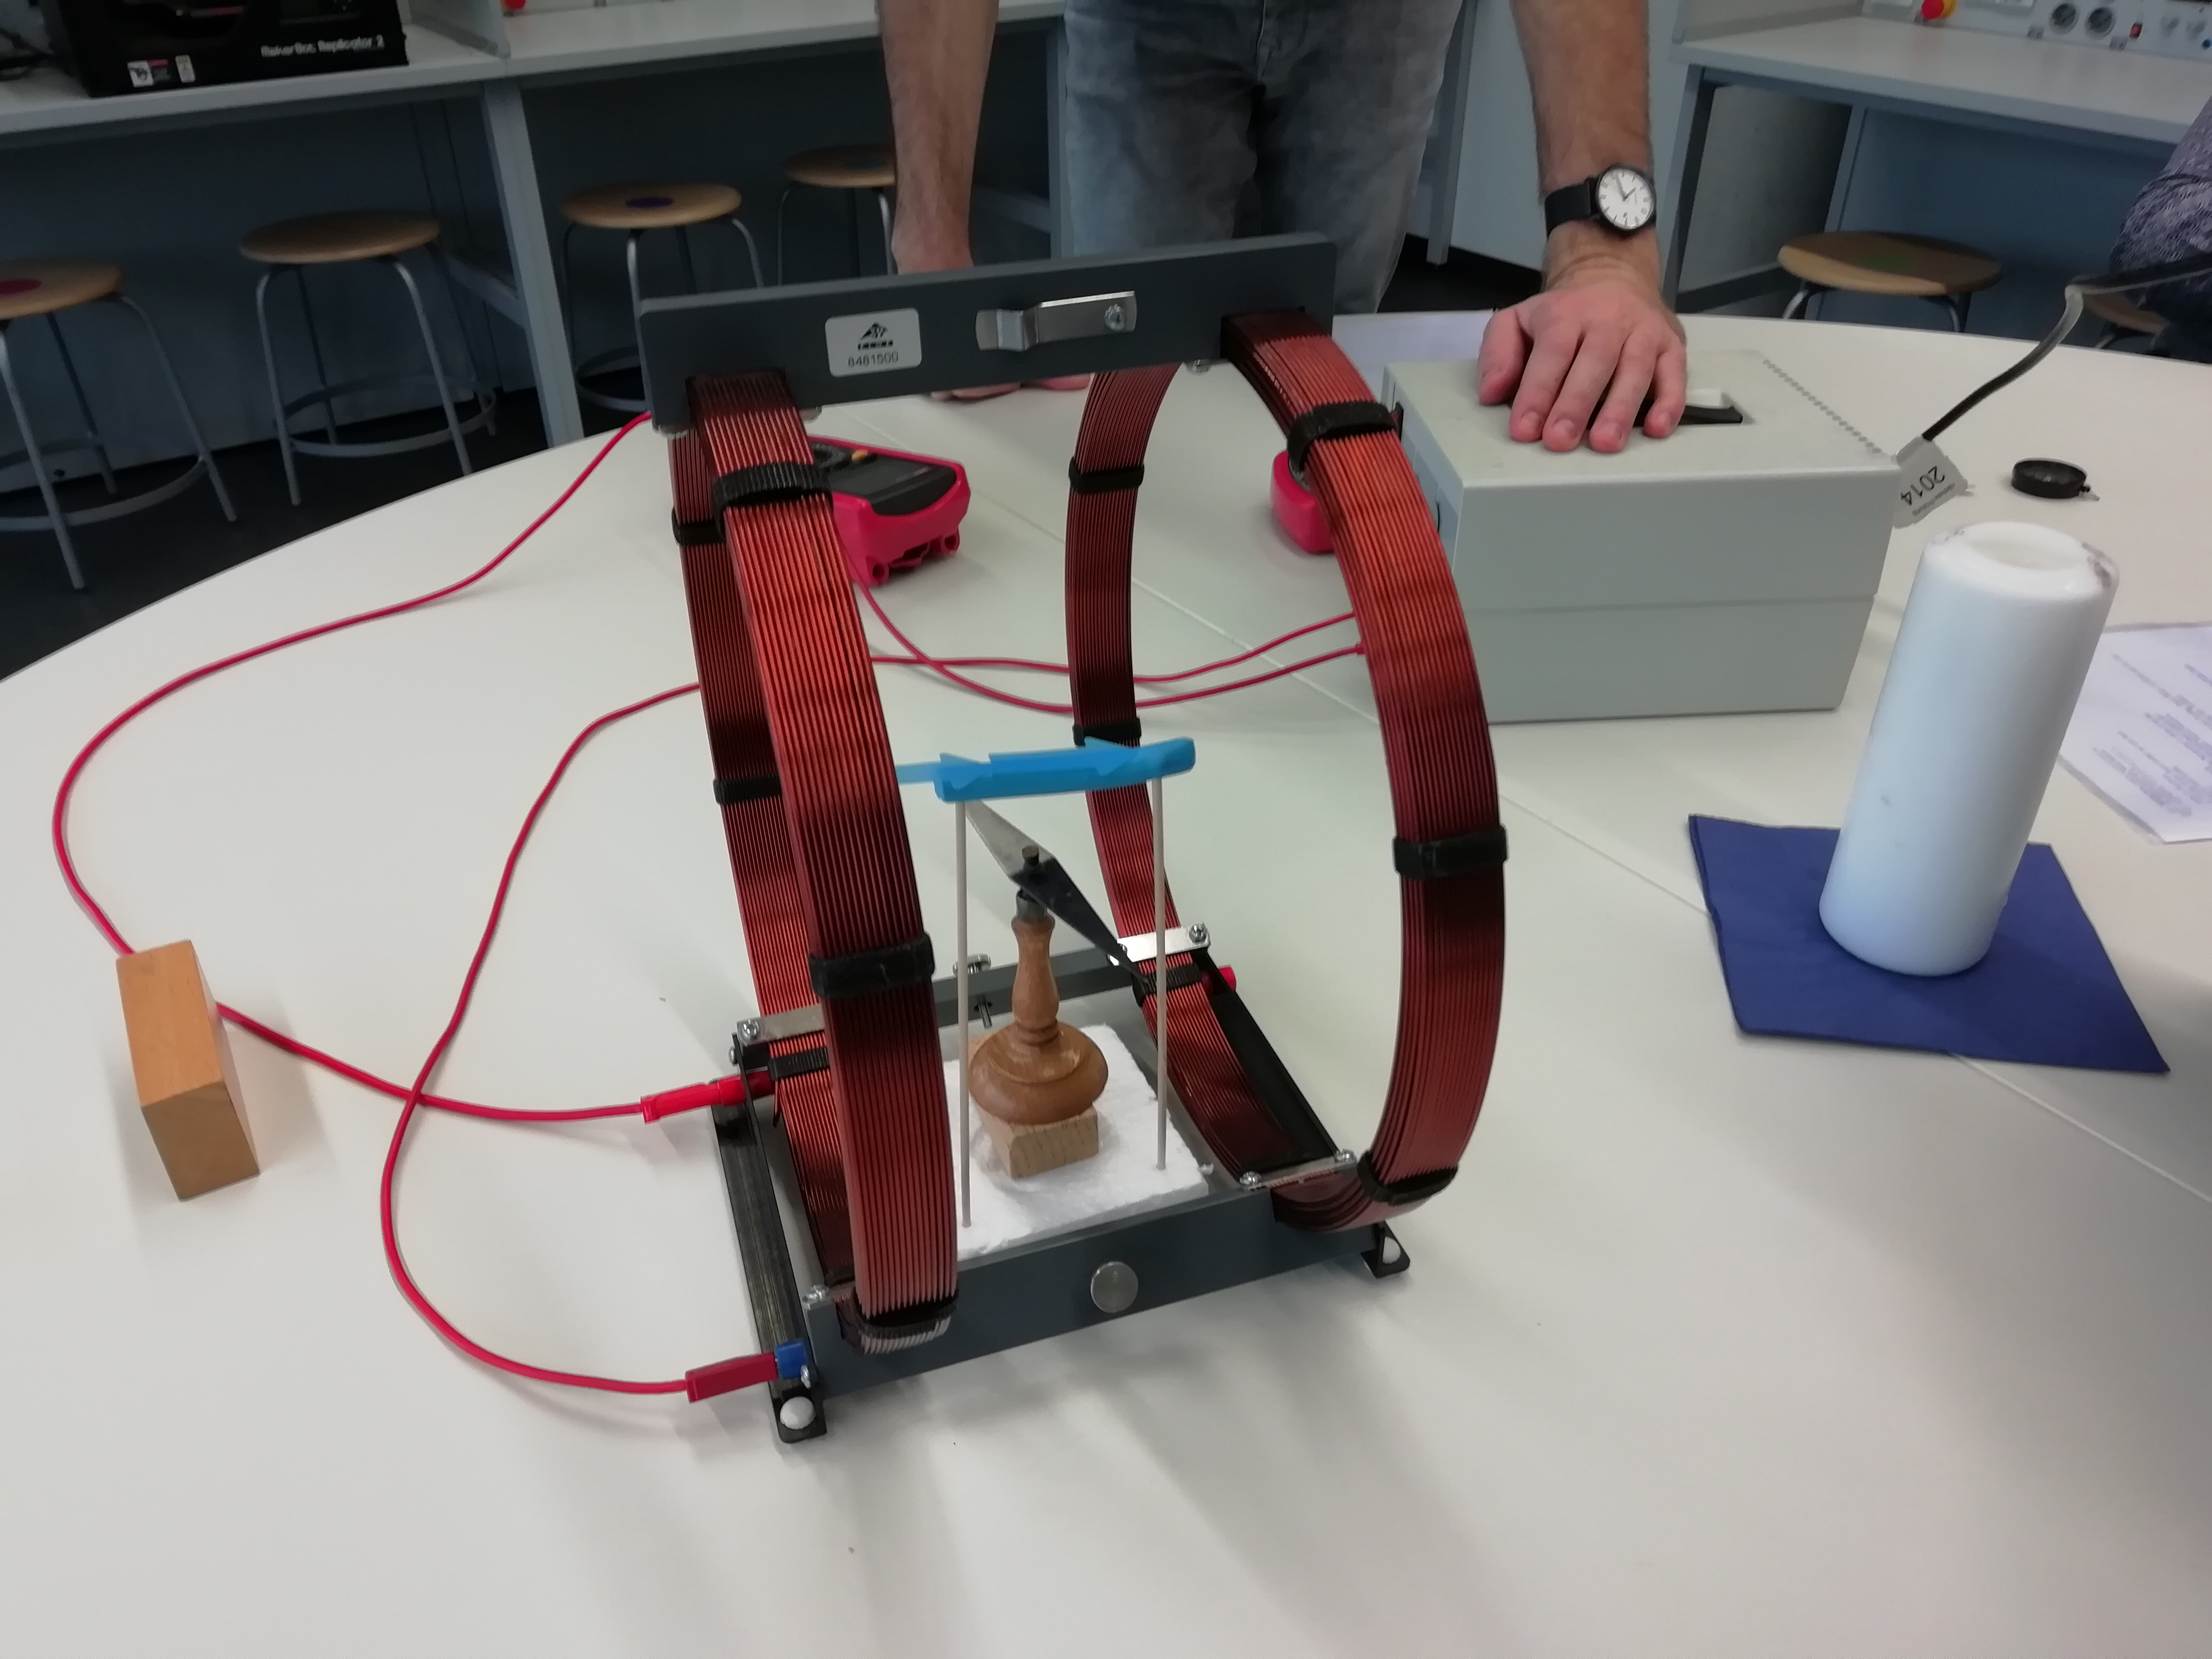
\includegraphics[width=0.8\textwidth]{images/Design_Magnetfeld.jpg}	
\end{center}
\end{frame}

\begin{frame}[fragile]{Vergleich mit Anforderungen}
\begin{itemize}
	\item Inhaltliche Anforderungen
	\item Distanz, Geschwindigkeit, Farbe von Objekten
	\item Keine Störung der Sensorik
	\item Keine Störung der Sensorik	
	
	\item Einbettung durch Depth Cues unterstützen (in erster Linie Verdeckung der virtuellen Geometrie durch reale Spule)
	\item Sensordaten in Echtzeit an HoloLens übermitteln und Geometrie auf dem Device in Echtzeit berechnen und darstellen
\end{itemize}
\end{frame}

\begin{frame}[fragile]{Ansatz -- Weitere Elemente }
\begin{itemize}
	\item Eingebetteter 3D-Kompass mit Markierungen anzeigen
	\item Statusinformationen als Text-UI Elemente anzeigen
	\item Stromfluss durch 2D Geometrie, verankert an den beiden Spulen-Teilen, visualisieren
\end{itemize}
\end{frame}


\part{Umsetzung und Ausblick}
\label{part:practice}

\begin{frame}[fragile]{}
ASDF
\end{frame}